% Options for packages loaded elsewhere
\PassOptionsToPackage{unicode}{hyperref}
\PassOptionsToPackage{hyphens}{url}
\documentclass[
  ignorenonframetext,
]{beamer}
\newif\ifbibliography
\usepackage{pgfpages}
\setbeamertemplate{caption}[numbered]
\setbeamertemplate{caption label separator}{: }
\setbeamercolor{caption name}{fg=normal text.fg}
\beamertemplatenavigationsymbolsempty
% remove section numbering
\setbeamertemplate{part page}{
  \centering
  \begin{beamercolorbox}[sep=16pt,center]{part title}
    \usebeamerfont{part title}\insertpart\par
  \end{beamercolorbox}
}
\setbeamertemplate{section page}{
  \centering
  \begin{beamercolorbox}[sep=12pt,center]{section title}
    \usebeamerfont{section title}\insertsection\par
  \end{beamercolorbox}
}
\setbeamertemplate{subsection page}{
  \centering
  \begin{beamercolorbox}[sep=8pt,center]{subsection title}
    \usebeamerfont{subsection title}\insertsubsection\par
  \end{beamercolorbox}
}
% Prevent slide breaks in the middle of a paragraph
\widowpenalties 1 10000
\raggedbottom
\AtBeginPart{
  \frame{\partpage}
}
\AtBeginSection{
  \ifbibliography
  \else
    \frame{\sectionpage}
  \fi
}
\AtBeginSubsection{
  \frame{\subsectionpage}
}
\usepackage{iftex}
\ifPDFTeX
  \usepackage[T1]{fontenc}
  \usepackage[utf8]{inputenc}
  \usepackage{textcomp} % provide euro and other symbols
\else % if luatex or xetex
  \usepackage{unicode-math} % this also loads fontspec
  \defaultfontfeatures{Scale=MatchLowercase}
  \defaultfontfeatures[\rmfamily]{Ligatures=TeX,Scale=1}
\fi
\usepackage{lmodern}
\ifPDFTeX\else
  % xetex/luatex font selection
\fi
% Use upquote if available, for straight quotes in verbatim environments
\IfFileExists{upquote.sty}{\usepackage{upquote}}{}
\IfFileExists{microtype.sty}{% use microtype if available
  \usepackage[]{microtype}
  \UseMicrotypeSet[protrusion]{basicmath} % disable protrusion for tt fonts
}{}
\makeatletter
\@ifundefined{KOMAClassName}{% if non-KOMA class
  \IfFileExists{parskip.sty}{%
    \usepackage{parskip}
  }{% else
    \setlength{\parindent}{0pt}
    \setlength{\parskip}{6pt plus 2pt minus 1pt}}
}{% if KOMA class
  \KOMAoptions{parskip=half}}
\makeatother
\usepackage{graphicx}
\makeatletter
\newsavebox\pandoc@box
\newcommand*\pandocbounded[1]{% scales image to fit in text height/width
  \sbox\pandoc@box{#1}%
  \Gscale@div\@tempa{\textheight}{\dimexpr\ht\pandoc@box+\dp\pandoc@box\relax}%
  \Gscale@div\@tempb{\linewidth}{\wd\pandoc@box}%
  \ifdim\@tempb\p@<\@tempa\p@\let\@tempa\@tempb\fi% select the smaller of both
  \ifdim\@tempa\p@<\p@\scalebox{\@tempa}{\usebox\pandoc@box}%
  \else\usebox{\pandoc@box}%
  \fi%
}
% Set default figure placement to htbp
\def\fps@figure{htbp}
\makeatother
\setlength{\emergencystretch}{3em} % prevent overfull lines
\providecommand{\tightlist}{%
  \setlength{\itemsep}{0pt}\setlength{\parskip}{0pt}}
% Slide layout defaults for warning-clean scientific decks.
\usepackage{etoolbox}
\IfFileExists{xurl.sty}{\usepackage{xurl}}{}
\IfFileExists{seqsplit.sty}{\usepackage{seqsplit}}{\newcommand{\seqsplit}[1]{#1}}
\protected\def\breakseq#1{\seqsplit{#1}}
\protected\def\breaktt#1{\begingroup\ttfamily\seqsplit{#1}\endgroup}
\setlength{\emergencystretch}{6em}
\tolerance=5000
\hbadness=10000
\hfuzz=1pt
\setlength{\tabcolsep}{2pt}
\AtBeginEnvironment{longtable}{\tiny\renewcommand{\arraystretch}{0.86}\setlength{\tabcolsep}{1pt}}
\AtBeginEnvironment{tabular}{\tiny\renewcommand{\arraystretch}{0.86}\setlength{\tabcolsep}{1pt}}

% Natbib and cross-reference fallbacks — slides don't load natbib
% or cleveref, but combined-PDF manuscript prose may emit these
% commands. The fallback renders citations as a bracketed key list
% and cross-references as detokenized labels so slides don't fail on
% undefined control sequences or raw underscores. \providecommand is
% a no-op if packages load later.
\providecommand{\citep}[1]{[#1]}
\providecommand{\citet}[1]{#1}
\providecommand{\citealp}[1]{#1}
\providecommand{\citeauthor}[1]{#1}
\providecommand{\citeyear}[1]{#1}
\providecommand{\cref}[1]{\texttt{\detokenize{#1}}}
\providecommand{\Cref}[1]{\texttt{\detokenize{#1}}}

\newtheorem{proposition}{Proposition}
\newtheorem{hypothesis}{Hypothesis}
\usepackage{bookmark}
\IfFileExists{xurl.sty}{\usepackage{xurl}}{} % add URL line breaks if available
\urlstyle{same}
% fallback for those not using the hyperref driver hyperxmp:
\makeatletter
\@ifundefined{xmpquote}{\newcommand{\xmpquote}[1]{#1}}{}
\makeatother
\hypersetup{
  hidelinks,
  pdfcreator={LaTeX via pandoc}}

\author{\texorpdfstring{}{}}
\date{}

\begin{document}

\section{Introduction: From Shared Marks to Study-Ready
Infrastructure}\label{sec:introduction}

\begin{frame}[fragile,allowframebreaks]{Introduction: From Shared Marks
to Study-Ready Infrastructure}
The original PPPiP paper defined a simple dyadic practice: two partners
draw simultaneously on one shared sheet, treating improvised mark-making
as a non-clinical, low-cost, relational exercise
\breakseq{[@mikhailova2018pppip]}. Couple joint-drawing research also gives the
manuscript a more direct arts-therapy precedent for reading
connectedness and individuality through shared image-making
\breakseq{[@snir2013joint]}. Its theoretical value came from the convergence of
art therapy, partner improvisation, controlled novelty, interpersonal
neural synchrony, and the Free Energy Principle \breakseq{[@friston2010fep]}.
DigiPPPiP keeps that foundation but asks what changes when the shared
surface becomes a tablet, networked canvas, augmented paper, persistent
whiteboard, or place-responsive archive.

The CSCW lineage matters because shared drawing surfaces have long been
more than image-output devices, and computer-supported cooperative work
(CSCW) supplies the analytic vocabulary for treating a shared surface as
an interaction scene rather than a delivery channel. Observational work
on collaborative drawing showed that gestures, spatial orientation,
drawing process, and the common workspace all carry information that the
finished drawing alone does not capture
\breakseq{[@tang1991collaborativework]}. ClearBoard made the same point
technologically by integrating interpersonal space with a shared drawing
workspace, using gaze and gesture as part of the collaborative medium
rather than as side channels \breakseq{[@ishii1993clearboard]}. Social
translucence and workspace-awareness research then name the design
obligation: a system should make relevant partner activity visible
enough to support awareness and accountability while avoiding
indiscriminate exposure \breakseq{[@erickson2000socialtranslucence;
@gutwin2002workspaceawareness]}. DigiPPPiP therefore treats the canvas
as an interaction scene: marks, pauses, attention shifts, access
controls, and return visits are part of the relational event. This
positioning prevents a novelty overclaim. The contribution is not that
digital co-drawing exists, but that PPPiP can be reframed as a
reproducible, partner-centered research program for studying how shared
marks mediate relational attention.

From first principles, the framework has fewer hard requirements than a
typical app description implies. It requires participating agents who
can affect a shared surface; a trace that both partners can perceive,
interpret, or revisit; enough temporal structure to distinguish
simultaneous, alternating, and delayed action; and governance over who
can save, replay, export, or erase the artifact. Tablets, augmented
reality (AR) overlays, machine-learning prompts, physiological sensors,
and cloud archives are optional implementations, not constitutive
requirements. This distinction matters because DigiPPPiP should not
optimize for digital sophistication when the function to preserve is
reciprocal attention through marks.

The project brief motivates a successor framework with cyberphysical,
temporal, active-inference, neuroergonomic, cyber-phenomenological,
accessibility, relational-aesthetic, place-based, and dyadic
digital-health dimensions. The evidence graph in
\breakseq{[@fig:evidence\_synthesis]} formalizes those dimensions as a lineage
from the original PPPiP domains into the present framework. The graph
currently covers 5 source domains and 13 DigiPPPiP dimensions with 100
percent citation coverage.

\begin{figure}
\centering
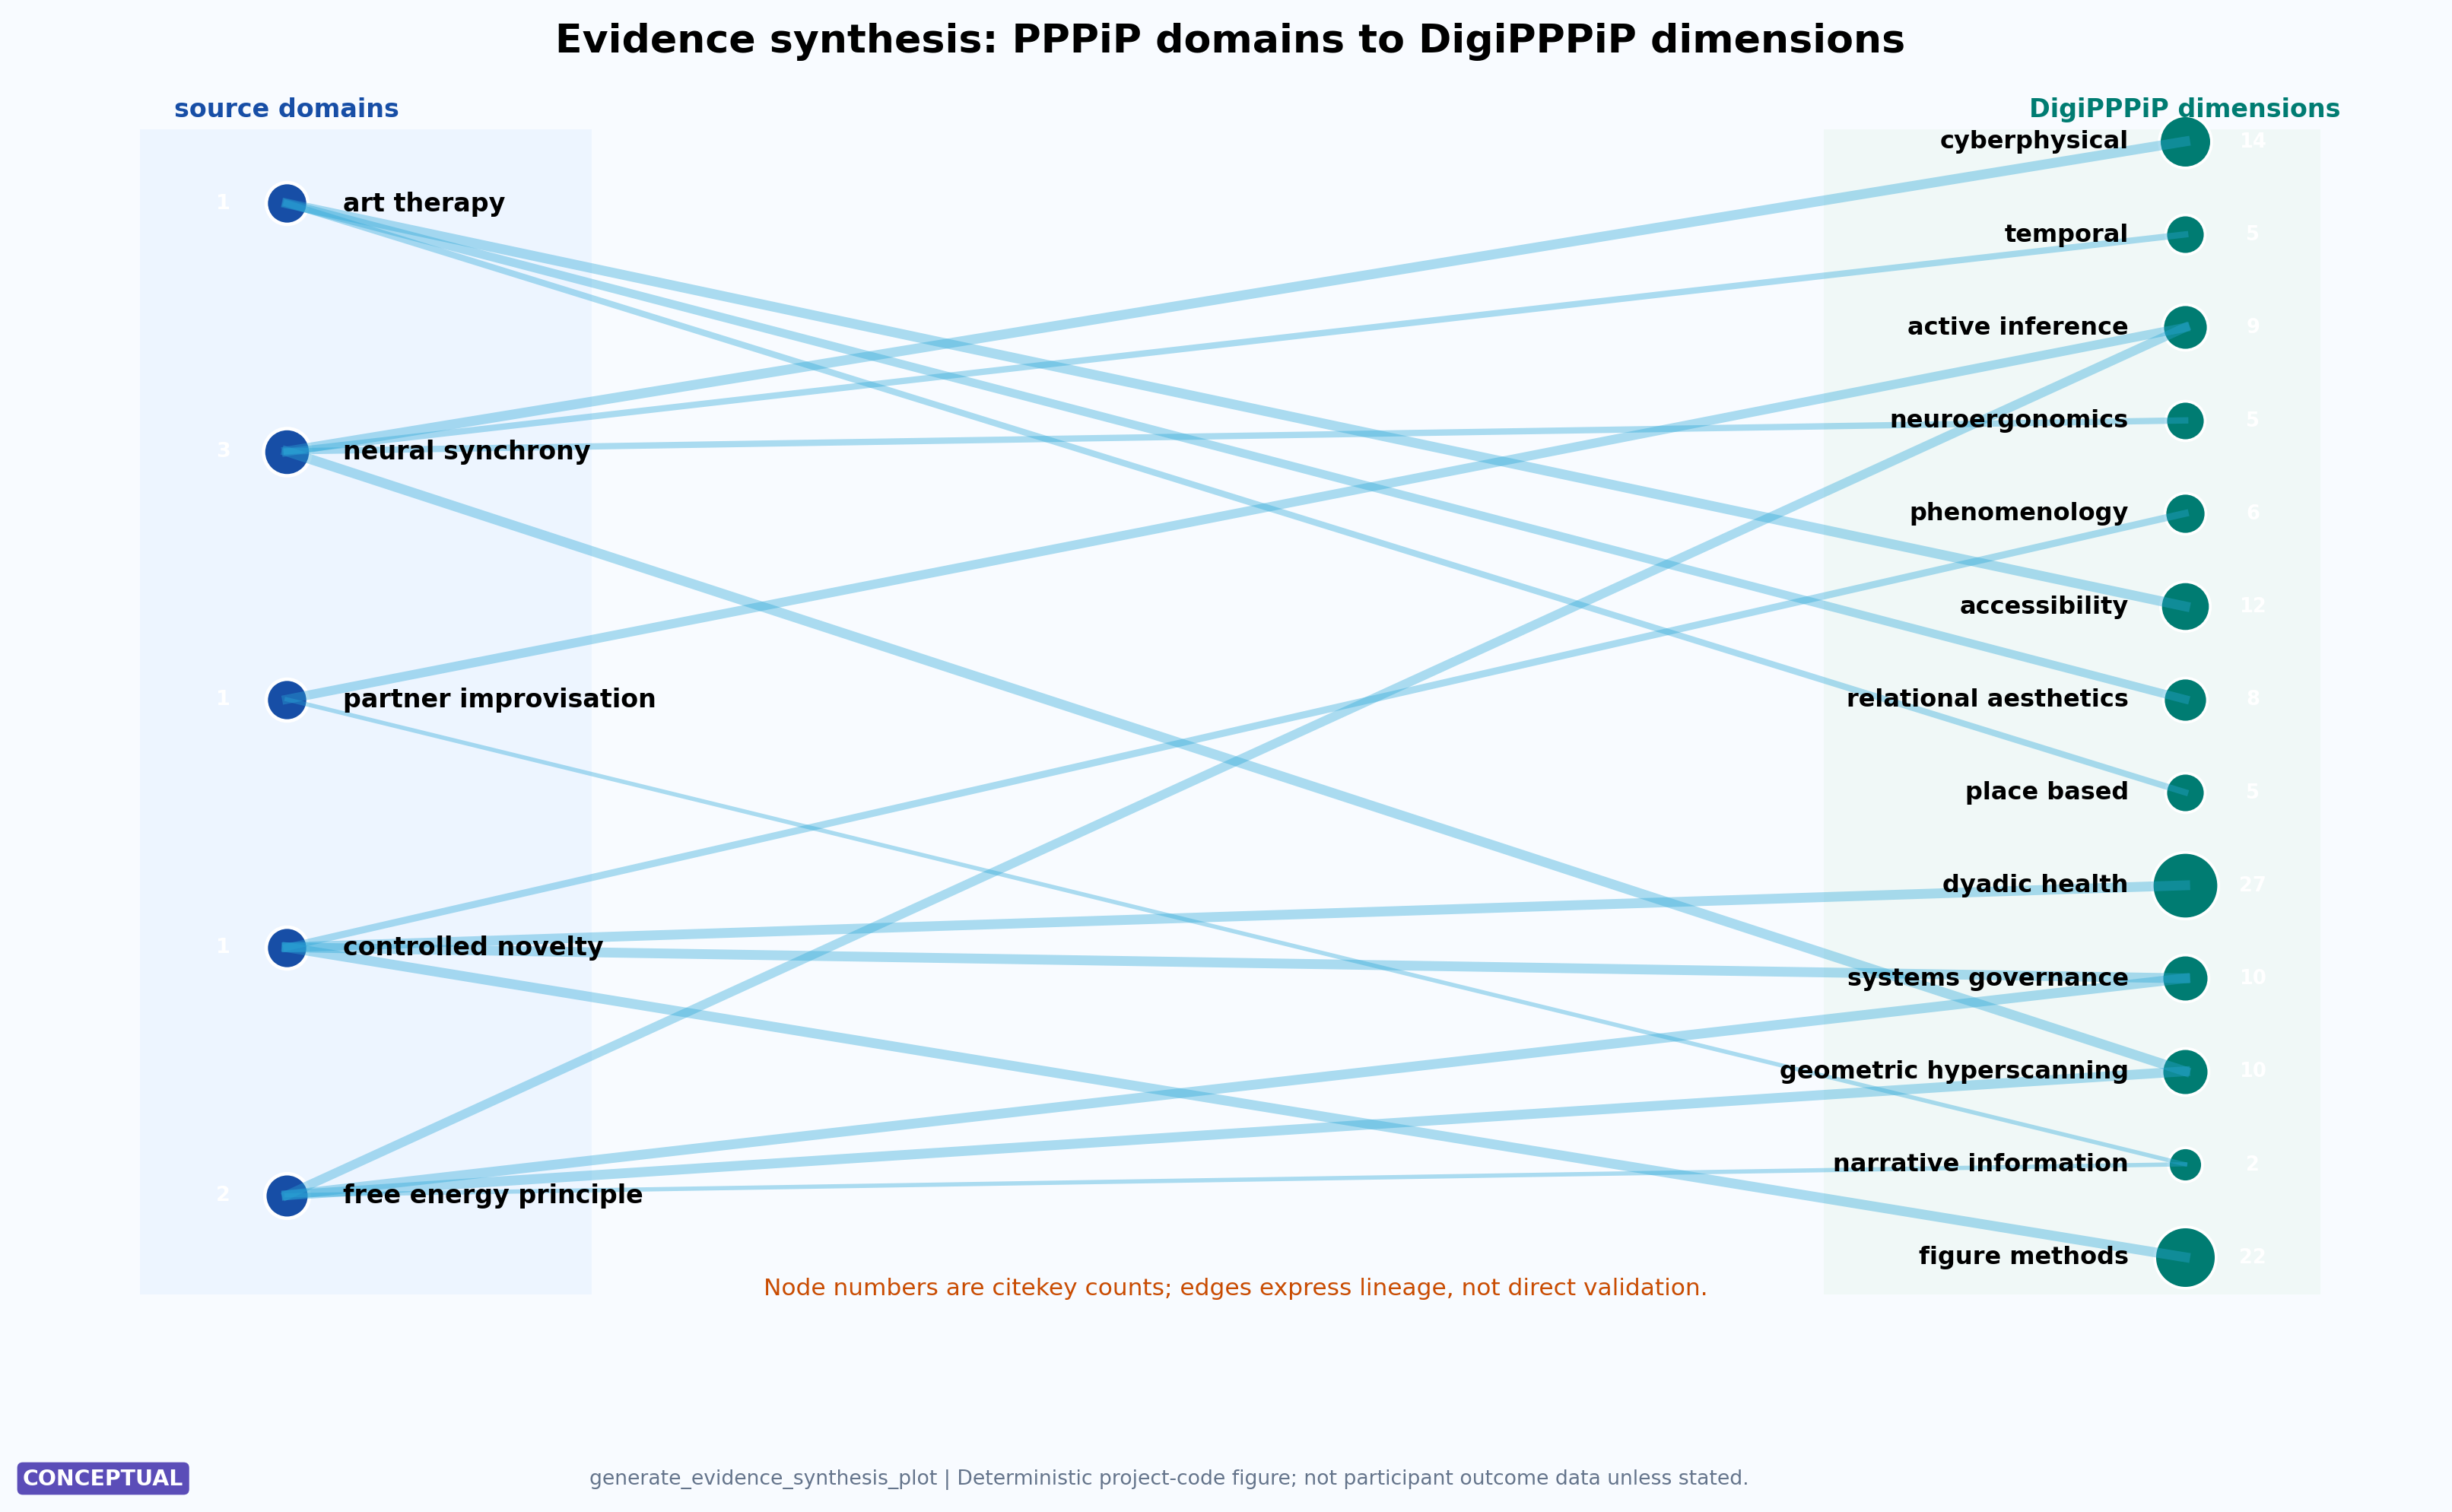
\includegraphics[width=0.9\linewidth,height=0.46\textheight,keepaspectratio,alt={Bipartite evidence graph linking original PPPiP evidence domains to DigiPPPiP dimensions. This conceptual synthesis is generated by generate\_evidence\_synthesis\_plot() from the citation-bearing graph in src/evidence.py; read left nodes as source domains, right nodes as framework dimensions, node numbers as citekey counts, and link weight as lineage density supporting the introduction's scope argument. It is conceptual rather than empirical, and stronger claims would require direct comparative studies within each dimension.}]{../figures/evidence_synthesis.png}
\caption{Bipartite evidence graph linking original PPPiP evidence
domains to DigiPPPiP dimensions. This conceptual synthesis is generated
by \protect\breaktt{generate\_evidence\_synthesis\_plot()} from the
citation-bearing graph in \protect\texttt{src/evidence.py}; read left
nodes as source domains, right nodes as framework dimensions, node
numbers as citekey counts, and link weight as lineage density supporting
the introduction's scope argument. It is conceptual rather than
empirical, and stronger claims would require direct comparative studies
within each dimension.}\label{fig:evidence_synthesis}
\end{figure}

DigiPPPiP is therefore a framework for designing and studying
intentional shared drawing across substrates. It is not a claim that
every digital canvas is therapeutic, nor that any synthetic model here
measures a real couple. A weak implementation would merely connect users
to drawing software; a stronger implementation would preserve agency,
mutual visibility, access, privacy, and interpretive openness. The
manuscript uses computational primitives to keep conceptual claims
explicit and testable: \breakseq{[@fig:evolution\_timeline]} shows the
conceptual expansion, \breakseq{[@fig:conceptual\_ecology]} maps the actors and
artifacts, \breakseq{[@sec:taxonomy]} defines the design space,
\breakseq{[@sec:active\_inference]} states the modeling lens,
\breakseq{[@sec:formalisms\_appendix]} keeps the formal primitives inspectable,
\breakseq{[@sec:methods\_protocol]} specifies what future studies must log and
govern, and \breakseq{[@sec:agenda]} names the empirical work required before
intervention claims would be justified.

Reader route map: substrate, temporal coordination, and taxonomy
sections define what counts as a DigiPPPiP condition; the modeling,
neuroergonomic, phenomenological, accessibility, aesthetic, and place
sections explain how the condition can be interpreted without treating
interpretation as evidence; the digital-health section sets the dyadic
ethics boundary; the methods protocol specifies source verification,
figure provenance, participant-facing controls, and validation gates;
the agenda and discussion sections state what evidence would strengthen
or falsify the framework. The route is intentionally ordered from theory
to protocol to limits, with the formal appendix separated so equations
and diagnostic figures do not outrun the human-human claim.

\begin{figure}
\centering
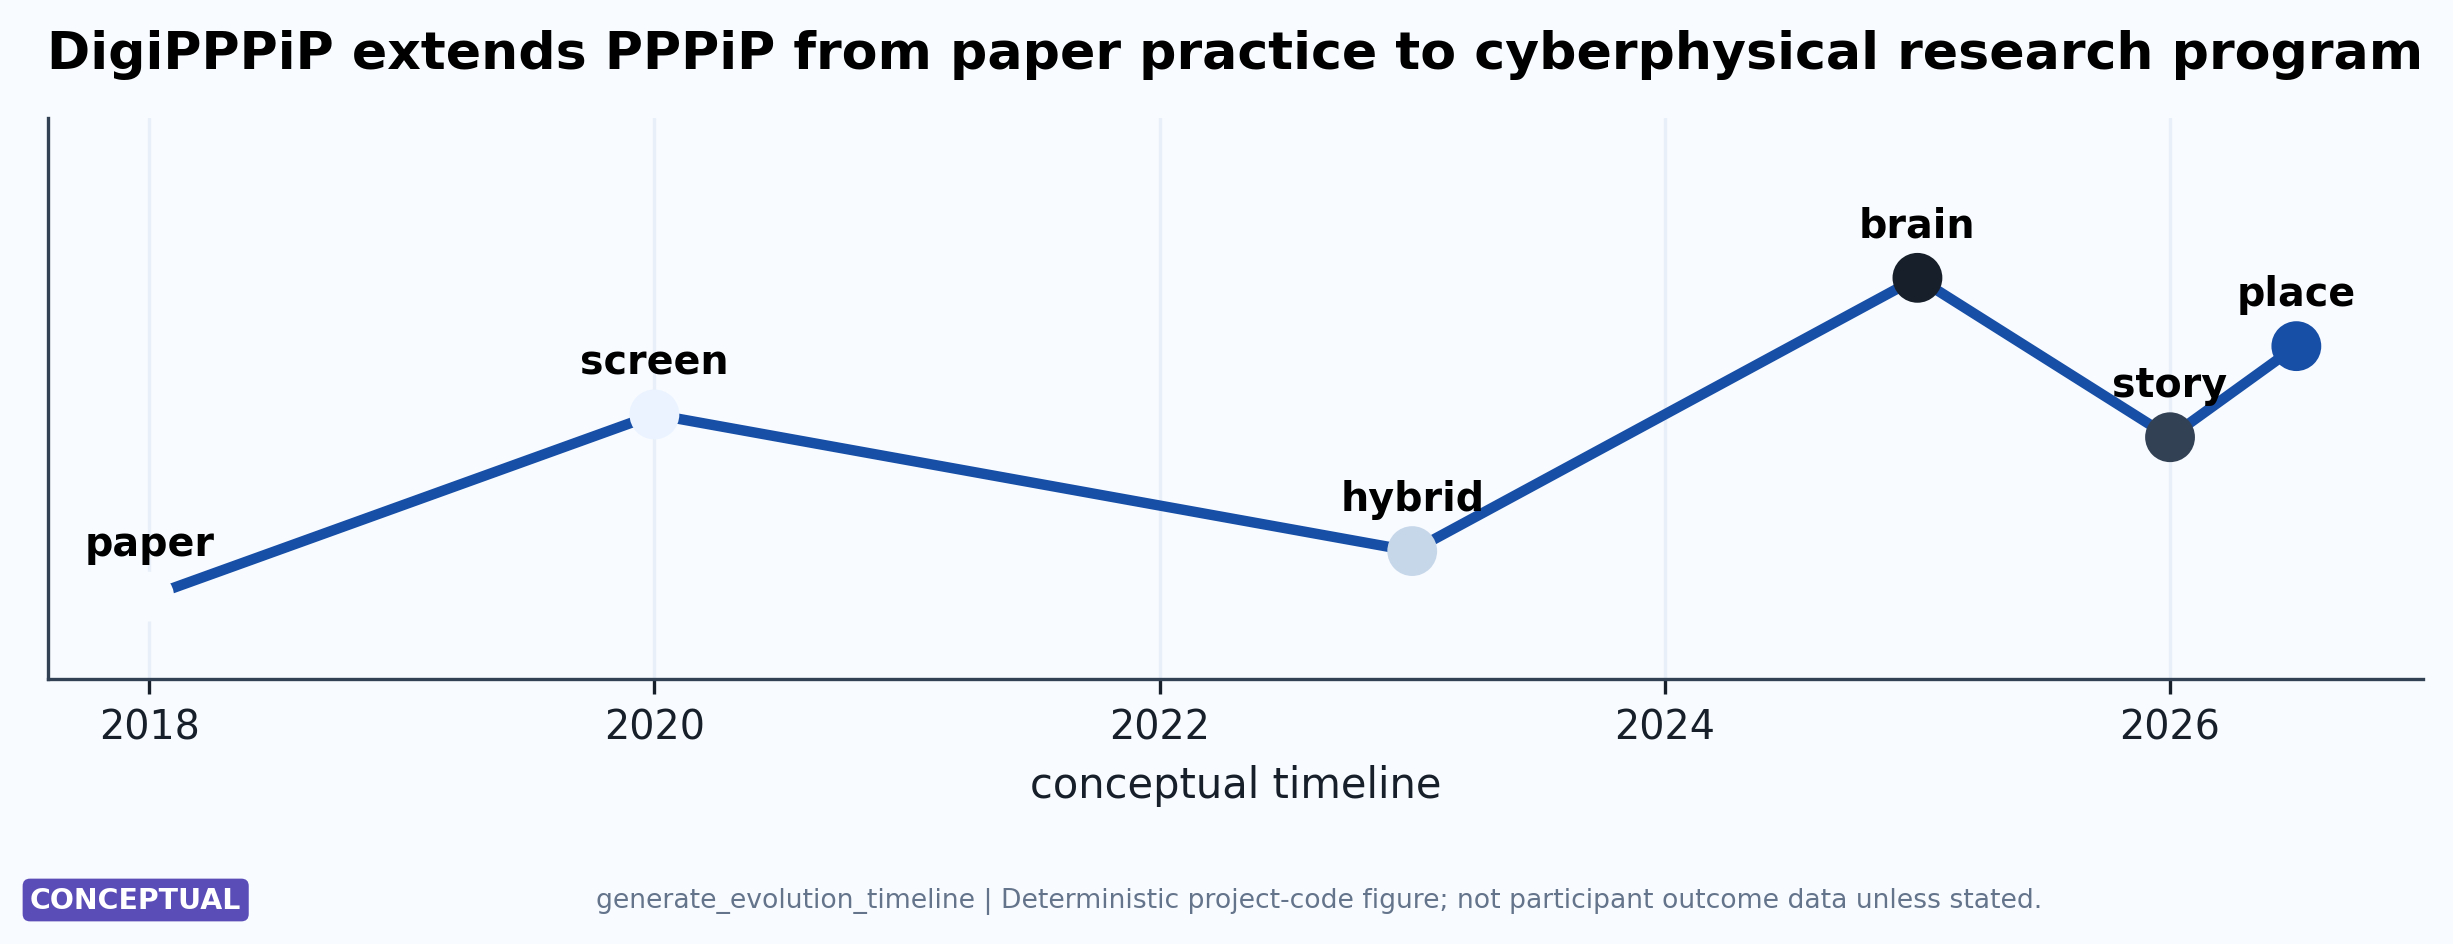
\includegraphics[width=0.9\linewidth,height=0.46\textheight,keepaspectratio,alt={Timeline of the conceptual expansion from paper PPPiP into a cyberphysical research program. The figure is generated by generate\_evolution\_timeline(); read the connected markers as staged additions of substrate, hybrid interaction, neural measurement, narrative analysis, and place responsiveness. It supports the introduction's claim that DigiPPPiP is an organized expansion, not an adoption history or outcome trend; empirical chronology would require archival or deployment data.}]{../figures/evolution_timeline.png}
\caption{Timeline of the conceptual expansion from paper PPPiP into a
cyberphysical research program. The figure is generated by
\protect\breaktt{generate\_evolution\_timeline()}; read the connected
markers as staged additions of substrate, hybrid interaction, neural
measurement, narrative analysis, and place responsiveness. It supports
the introduction's claim that DigiPPPiP is an organized expansion, not
an adoption history or outcome trend; empirical chronology would require
archival or deployment data.}\label{fig:evolution_timeline}
\end{figure}

\begin{figure}
\centering
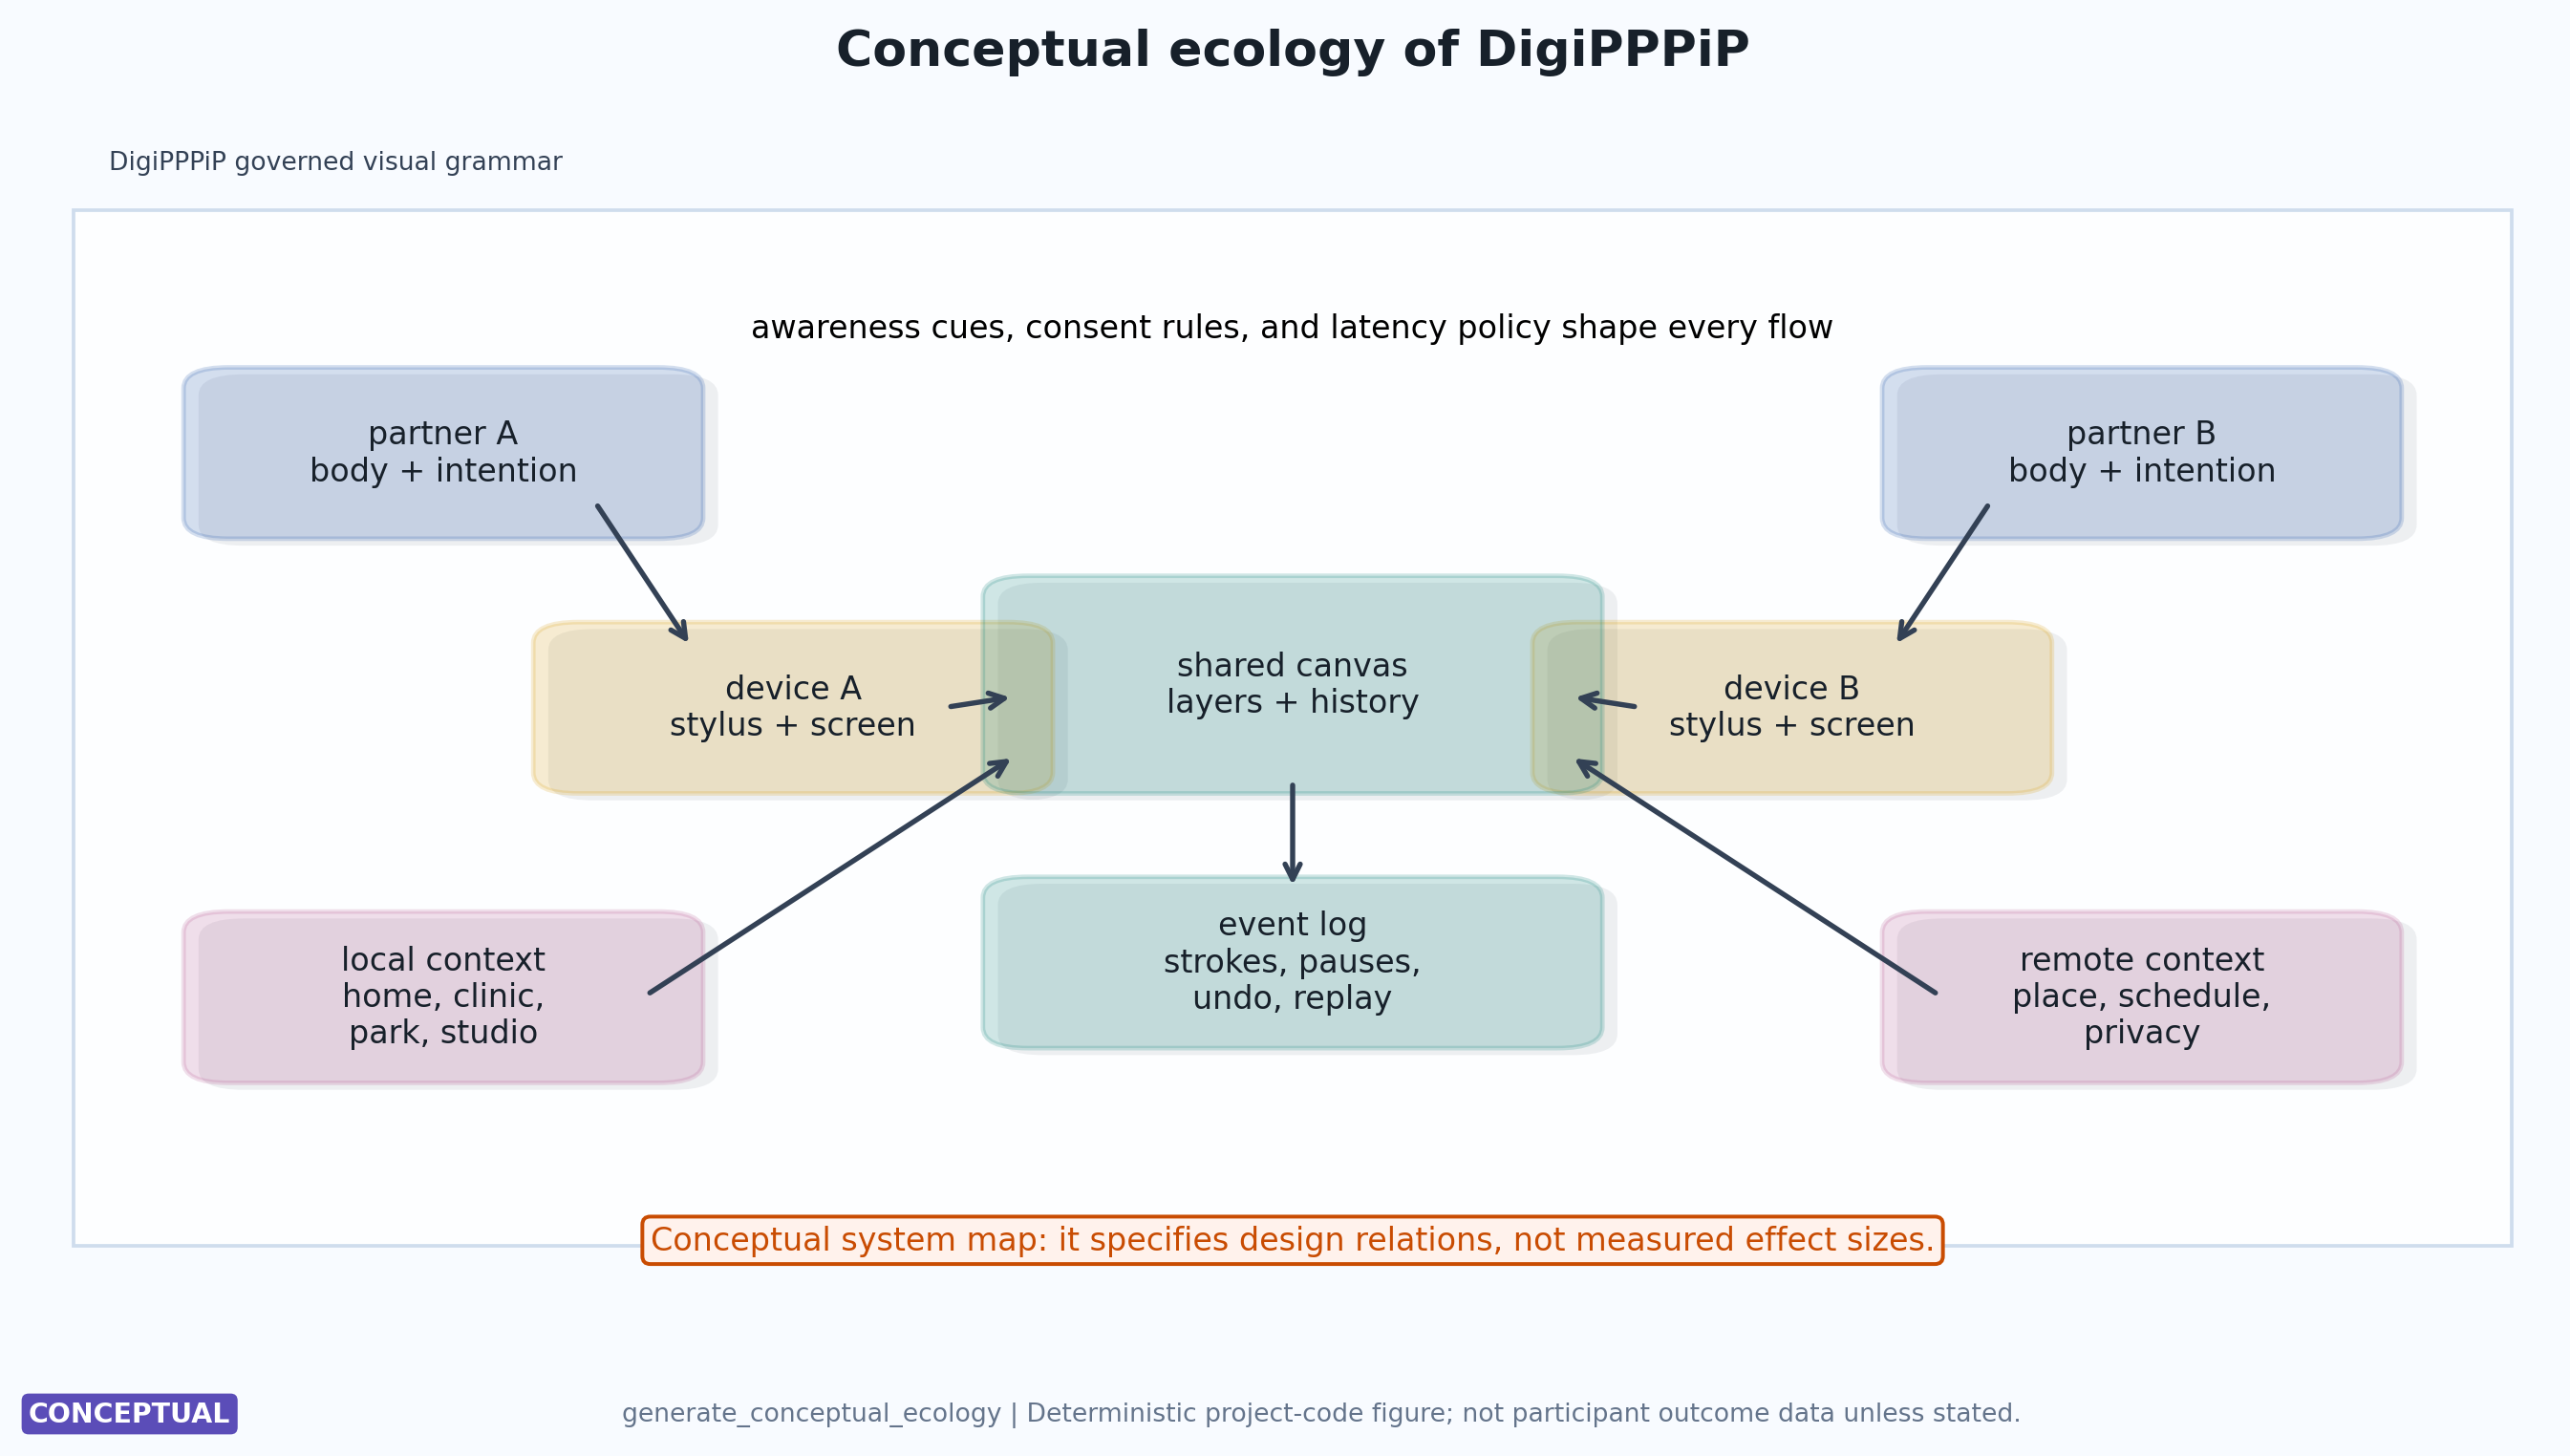
\includegraphics[width=0.9\linewidth,height=0.46\textheight,keepaspectratio,alt={Conceptual ecology of DigiPPPiP as a dyadic system of actors, devices, shared canvas artifacts, event logs, and situated contexts. The visual grammar is generated by generate\_conceptual\_ecology(); blue actor boxes, green artifact boxes, orange signal boxes, and purple context boxes show how partner agency flows through the shared surface. It supports the introduction's design-kernel argument and remains conceptual until instrumented sessions test these dependencies.}]{../figures/conceptual_ecology.png}
\caption{Conceptual ecology of DigiPPPiP as a dyadic system of actors,
devices, shared canvas artifacts, event logs, and situated contexts. The
visual grammar is generated by
\protect\breaktt{generate\_conceptual\_ecology()}; blue actor boxes,
green artifact boxes, orange signal boxes, and purple context boxes show
how partner agency flows through the shared surface. It supports the
introduction's design-kernel argument and remains conceptual until
instrumented sessions test these
dependencies.}\label{fig:conceptual_ecology}
\end{figure}
\end{frame}

\end{document}
